\section{View types}

In this section, we develop techniques for maintaining the following
basic view types in our VMS: \texttt{SELECTION}, \texttt{PROJECTION},
\texttt{INDEX}, aggregation (i.e. \texttt{COUNT}, \texttt{SUM},
\texttt{MIN}, \texttt{MAX}, \texttt{AVG}) and join
(i.e. \texttt{INNER}, \texttt{LEFT}, \texttt{RIGHT},
\texttt{FULL}). Internally, VMS provides a number of auxiliary views,
which are the \texttt{DELTA}, \texttt{PRE-AGGREGATION} and
\texttt{REVERSE-JOIN} view, described
shortly. Figure~\ref{fig:view_types} gives an overview of all view
types and their dependencies.

\begin{figure}
  \centering
    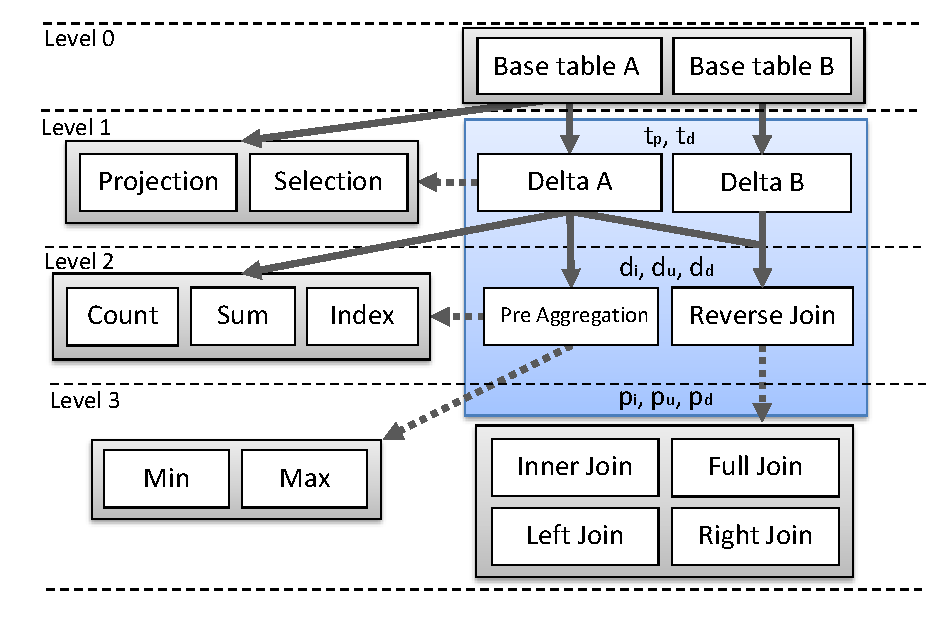
\includegraphics[width=\linewidth]{figures/ViewDependencies}
    \caption{View types and their dependencies}
    \label{fig:view_types}
\end{figure}



Views at Level~1 directly derive from base tables residing at Level~0,
as indicated by the directed edges in the figure. A path along edges
from a base table to a view at a higher-numbered layer represents a
complete update path through the system.  More complex views on
Level~2 and higher are derived from views on lower layers, which, from
the perspective of these views, serve them as ``base data''.  Note
that there are alternatives in how certain view types can be
derived. For example, \texttt{SELECTION} can be derived from a base
table or from a \texttt{DELTA} view. Determining
and quantifying the trade-offs among these view maintenance
alternatives is outside the scope of the present work. 

%
%Dotted edges indicate that a
%view type does not necessarily need to be materialized, as its
%deriving table provides sufficient information to materialize the
%given view on-the-fly without needing to scan table rows.  


%
%In our below description, we use the extended relational algebra
%notation to define views and update programs. View managers are
%triggered by base table updates, which are submitted by clients. These updates are
%denoted by $t_p$ and $t_d$ for put and delete, respectively, and $t_i$
%and $t_u$ for insert and update, respectively.

\subsection{Auxiliary views}
\label{subsec:auxiliary_views}

%Reasoning auxiliaries
Auxiliary views are internal to VMS and are not exposed to clients.
They are maintained to enable, facilitate and speed up the correct
maintenance of other view types.  Some views could not be maintained
consistently without the additional information provided by these
auxiliaries, others simply benefit from their pre-computations.  While
auxiliaries introduce storage overhead, they support modularity in 
view maintenance. Logically, auxiliaries represent the basic elements 
of view maintenance, which can be shared within and between view 
definitions. Thus, their use amortizes  as more
complexer views are managed by VMS. Auxiliaries also speed up view 
maintenance significantly. 
The update programs that compute the different view types make up most
of the view manger logic. 

%Auxiliary Table
In what follows, we describe each auxiliary view type, including the 
problem it solves and how it is maintained given base data updates.
In Table~\ref{tab:auxiliary_computation}, the definition, record format
and update operation of the auxiliary views are depicted. In the first
row the base table is shown. The records of the base table correspond
to the general format $r$. A client put (insert or update)
creates an update operation $t_p$, whereas a client delete creates a
$t_d$ operation. As discussed before, the KV-store updates the base
table by itself and provides operations $t_p$ and $t_d$ through the TL. 


\begin{table*}
\rowcolors{2}{gray!10}{gray!30}
\setlength{\belowrulesep}{0pt}
\setlength{\aboverulesep}{0pt}
\setlength\extrarowheight{2pt}
\begin{center}
\begin{tabular}{l l l l l}
\toprule
View type& Def & record format & on Insert & on Delete \\
\midrule
Base &$A$ & $r=(k,\{\langle c_1,v_1\rangle,..,\langle c_n, v_n\rangle\})$&$t_p=put(r)$&$t_d=delete(k)$  \\
Delta &$D=\delta(A)$ &  $r'=(k,\{\langle c_1,v_1'\rangle,..,\langle c_n, v_n'\rangle\})\lor \emptyset$&$put(r)$&$delete(k)$  \\
Pre Agg &$P=\gamma_{c_{\alpha},\langle K,c_{\beta}\rangle}(D)$ & $p=(v_{\alpha},\{\langle k_1, v_1\rangle,..,\langle k_n, v_n\rangle\})$& $put(v_{\alpha},\{\langle k,v_{\beta}\rangle\})$&$delete(v_{\alpha},\{k\})$  \\
Rev Join &$ R=\gamma_{c_{\alpha},\langle K,r\rangle,\langle L,s\rangle}(D_A, D_B)$ & $p=(v_{\alpha},\{\langle k_1,r_1\rangle,..,\langle k_n,r_n\rangle \}_A,..$&$A:put(v_{\alpha}\{\langle k,v_1\rangle\}_A)$&$A:delete(v_{\alpha},\{k\}_A)$  \\
 &  & $\{\langle l_1,s_1\rangle,..,\langle l_m, s_m\rangle \}_B)$&$B:put(v_{\alpha},\{\langle k,v_1\rangle\}_B)$&$B:delete(v_{\alpha},\{k\}_B)$ \\
\bottomrule 
\end{tabular}
\caption{Auxiliary computation}
\label{tab:auxiliary_computation}
\end{center}
\end{table*}


 



%Reasoning delta view
\noindent  
\textbf{Delta --} The \texttt{DELTA} view is an auxiliary view that 
tracks base table changes between successive update operations. TL 
entries only contain the client operation. They do not characterize the 
base record state before or after the operation. For example, for a 
delete operation, the client only provides the row key, but not the 
associated value to be deleted, as input. Likewise, an update operation 
provides the row key and new values, but not the old values to be 
modified. In fact, a TL entry does not distinguish between an insert and 
update operation. However, for view 
maintenance, this information is vital. This motivated us to introduce 
the \texttt{DELTA} view. It records base table entry changes, tracking 
the states between entry updates, i.e., the ``delta'' between two 
successive operations for a given row. Views that derive, have this 
information available for their maintenance operations. Now, we show 
the computation steps of the \texttt{DELTA} view when updated (see 
Table~\ref{tab:auxiliary_computation}).

%Computation delta view
\noindent
\textit{Computation:} The \texttt{DELTA} view is 
defined over the base table as $D_A=\delta(A)$, meaning all operations 
on the base table are forwarded to the view. The format of the records 
in $D_A$ corresponds to $r'$ -- the state of record $r$ before update 
operation $t_d$ or $t_p$ is applied (e.g. $r'$ holds the values that 
$t_d$ deletes; or $r'$ maybe $\emptyset$ if $t_p$ is an insert 
operation). Once $r'$ is retrieved from the \texttt{DELTA} view, $r$ 
becomes the new $r'$. The VMS updates the view accordingly. If the 
client operation was a delete ($t_d$), the VMS also deletes the record 
in the view. 




%Reasoning pre agg view
\noindent  
\textbf{Pre-Aggregation --} The \texttt{PRE-AGGREGATION} view is an 
auxiliary view that prepares the aggregation by already sorting and 
grouping the base table rows. Consecutive aggregation views only need 
to apply their aggregation function, then. Often, an application 
calculates different aggregations over the same aggregation key.  To materialize these
views, VMS must fetch the same record over and over. For \texttt{MIN}
and \texttt{MAX} views, the deletion of the minimum (maximum) in the
view requires an expensive base table scan to determine the new
minimum (maximum).  This motivated us to introduce the
\texttt{PRE-AGGREGATION} view. This view type sorts the base table
records according to the aggregation key, but stores the grouped rows
in a map.

%Computation pre agg
\noindent
\textit{Computation:}The \texttt{PRE-AGGREGATION} view $P$ is defined over the 
\texttt{DELTA} view $D$ (see Table~\ref{tab:auxiliary_computation}). The 
grouping of the view is based on a column name $c_a$ from the base 
records; the table of the view is sorted according to the grouping key 
$v_{\alpha}$. Every record in the view stores a map of key-value pairs 
(row key $k$ and grouping value $v_{\beta}$) -- representing the 
expanded list of grouping values that belong to a grouping key. The VMS 
can collapse this map in a second step to evaluate the count, sum, 
minimum, maximum or average of the grouped values. A pre-aggregation can 
only be defined over a \texttt{DELTA} view; an update may change the 
grouping key and, thus, requires touching the old and the new record in 
the view. 





%Reasoning reverse join view
\noindent  
\textbf{Reverse Join --}  A 
\texttt{JOIN} view is derived from at least two base tables. For an 
update to one of these tables, the VMS needs to query the other base 
table to determine the matching join rows. Only if the join-attribute is 
the row key of the queried base table, can the matching row be 
determined quickly, unless of course, an index is defined on the 
join-attribute for the table. Otherwise, a scan of the entire table is 
required, which has the following drawbacks: (i) Scans require a 
disproportional amount of time, slowing down view maintenance. (With 
increasing table size, the problem worsens.) (ii) Scans keep the nodes 
occupied, slowing down client requests. (iii) While a scan is in 
progress, underlying base tables may change, thus, destroying view data 
consistency for derived views. To address these issues, we introduce 
the \texttt{REVERSE-JOIN} view. It is an auxiliary view that supports 
the efficient and correct materialization of equi joins in VMS. 
\footnote{We are not discussing theta joins with a full join predicate, 
for it is outside the context of this work.} 

 
%computation reverse join view
\noindent
\textit{Computation (2-tables):}
A \texttt{REVERSE-JOIN} view supports the maintenance of a join between 
two tables: $A \bowtie B_{A.c_{\alpha}=B.c_{\alpha}}$, with join key in 
column $c_{\alpha}$ of tables $A$ and $B$. We define the \texttt{REVERSE
-JOIN} view analogous to the \texttt{PRE-AGGREGATION} view (see Table~
\ref{tab:auxiliary_computation}). This opens up
potential for savings in storage and computation; we can just use the 
same view for both view types (if grouping and join key are the same).

To build the view, we use an aggregation function that collects all 
records of a specific join key; the
join key, defined as $c_a$ -- full-filling the same purpose as the 
grouping key before -- becomes the row key of the view. However, in 
contrast to the \texttt{PRE-AGGREGATION} view, the \texttt{REVERSE-JOIN} 
view consumes tuples from two different input tables, namely $D_A$ and 
$D_B$. When updates are propagated, the
\texttt{REVERSE-JOIN} view can be accessed rapidly from either side of the
relation (the join key is always included in both
tables' updates). If a record is inserted into one of the underlying
base tables, it is stored into the view --- whether it has a
matching row in the join table or not. We are using column families $\{..\}A$ and $\{..\}B$ in the view
to distinguish updates from different base tables. Later, this
facilitates the computation of the matching join rows, for we only
need to build the cross product between the records of the families.  Thus, \texttt{INNER}, 
\texttt{LEFT}, \texttt{RIGHT}, and \texttt{FULL JOIN} can derive from the 
\texttt{REVERSE-JOIN} view without the need for base table scans, as 
we show below.  We discussed the \texttt{REVERSE JOIN} with two join 
tables and a single join key. When increasing the number of join tables
to $n$,  we distinguish two cases:   

(i) Join all tables on the same join key: we just need to extend the
prior definition to $n$ tables. For every new join table $\Phi$ with \texttt{DELTA} view
$D_{\Phi}$, a new column family is added to the view. This column
family collects the updates of the base table.  As long as we are
joining on the same key, we can put all relations to the same
\texttt{REVERSE-JOIN} view.

(ii) base tables are joined on different join keys: for
example, $A \bowtie B \bowtie C$, where table $A$ and $B$ are joined
on column $c_1$, whereas table $B$ and $C$ are joined on a column
$c_3$.  To enable this, we have to combine multiple
\texttt{REVERSE-JOIN} views. We are free to choose, whether we build a
\texttt{REVERSE-JOIN} for $A \bowtie B$ and combine the result with
$C$ or we build a \texttt{REVERSE-JOIN} for $B \bowtie C$ and combine
it with $A$. For every pair of distinct join keys, we need a
\texttt{REVERSE-JOIN} view.  In the worst case, we have $n$ join
tables and $n-1$ distinct join keys, resulting in the same number of
\texttt{REVERSE-JOIN} views.  However, this compositional manner of
deriving join views, leads to a number of possible optimizations. When
computing join $A \bowtie B \bowtie C$ and $B \bowtie C \bowtie D$,
relation $B \bowtie C$ only needs to be computed once, for instance.



\subsection{Standard views}
\label{subsec:common_views}


\begin{table*}
\rowcolors{2}{gray!10}{gray!30}
\setlength{\belowrulesep}{0pt}
\setlength{\aboverulesep}{0pt}
\setlength\extrarowheight{2pt}
\begin{center}
\begin{tabular}{l l l l l}
\toprule
View type & Def & record format & Insert & Delete \\
\midrule
Selection &$\sigma_{C}(D)$  & $r \lor \emptyset$&$(C)\rightarrow put(r)$&$(C)\rightarrow delete(k,\{c_1,..,c_n\})$  \\
Projection &$\pi_{c_{\alpha_1},..c_{\alpha_n}}(D)$&  $(k,\{\langle c, v\rangle \mid c \in {c_{\alpha_1},..c_{\alpha_n}}\})$&$put(k,\{\langle c, v\rangle \mid c \in {c_{\alpha_1},..c_{\alpha_n}}\})$&$delete(k,\{c_{\alpha_1},..,c_{\alpha_n}\})$  \\
Count &$\gamma_{c_{\alpha},Count(c_{\beta})}(D)$ & $(v_{\alpha},\{\langle c, v_{count}\rangle\})$& $put(v_{\alpha},\{\langle c,v_{count} + 1\rangle\})$&$put(v_{\alpha},\{\langle c,v_{count} - 1\rangle\})$  \\
Sum &$\gamma_{c_{\alpha},Sum(c_{\beta})}(D)$& $(v_{\alpha},\{\langle c, v_{sum}\rangle\})$& $put(v_{\alpha},\{\langle c,v_{sum} + v_{\beta}\rangle\})$&$put(v_{\alpha},\{\langle c,v_{sum} - v_{\beta}\rangle\})$  \\
Min &$\gamma_{c_{\alpha},Min(c_{\beta})}(D)$& $(v_{\alpha},\{\langle c, v_{min}\rangle\})$& $(v_{\beta}<v_{min})\rightarrow put(v_{\alpha},\{\langle c,v_{\beta}\rangle\})$& $(v_{\beta}=v_{min})\rightarrow put(v_{\alpha},\{\langle c,v_{x}\rangle\})$ \\
Index &$\gamma_{c_{\alpha}}(D)$ & $v_{\alpha},\{\langle k_{\alpha},v_{\alpha}\rangle,..\}_A$&$put(\{\langle k,v_1\rangle\}_A)$&$delete(x,\{k\}_A)$  \\
Join &$A \bowtie B(R)$& $((k_{\alpha}),\{\langle k_{\alpha},v_{\alpha}\rangle,..\}_A$&$put(\{\langle k,v_1\rangle\}_A)$&$delete(x,\{k\}_A)$  \\
\bottomrule 
\end{tabular}
\caption{Standard computation}
\label{tab:kvs_a_events}
\end{center}
\end{table*}


In this section, we describe how VMS maintains client-exposed views
for a number of interesting standard view types. We also present
alternative maintenance strategies, but defer a full-fledged cost
analysis to future work.

\noindent  
\textbf{Selection and Projection --} A \texttt{SELECTION} view selects
a set of records from a base table based on a \textit{selection
  condition}.  The row key of the base table serves as the row key of
the view table and a single base record uniquely maps to a single view
table record.  

Let a selection view be defined as $S=\sigma_{c_2 <
  v_x}(A)$, where the selection condition is $(c_2 < v_x)$ requiring
that selected values in column $c_2$ are smaller than $v_x$.  The view
manager processes operations $t_p$ and $t_d$ as follows:
%
%\begin{eqnarray}
%	t_p & \Rightarrow & t_d\;\land\;\;(v_2 < v_x)\;\; \texttt{?} \;\;put(S(k_1,\langle c_1,v_1\rangle, \langle c_2,v_2\rangle))\\
%	t_d & \Rightarrow & delete(S(k))
%\end{eqnarray}
%
% aj - above - let us verify the notation, why use t_d and also delete(S(K))
% ja - I just want to point to the delete (no redundancy). Below are cases,
%	   where the t_d is very long and i don't want to repeat the whole op
A record delete is performed for every operation on the view.  This is
because, the selection condition cannot be evaluated on the operation,
as it may not contain the value.  For $t_d$, the VM does not know the
deleted value and cannot determine, if there is a corresponding view
record. For $t_p$, the VM is not able to distinguish between an insert
vs. an update.  Thus, in both cases, the VM pre-emptively deletes the
record in the view.



%Selection&&$\sigma_{c_{\alpha}<10}$& $r$ & $r \lor \emptyset$  \\
%Projection&&$\pi_{c_{\alpha_1},..,c_{\alpha_n}}$ & $r$ & $r \setminus \{\langle c_{\alpha_1},v_{\alpha_1}\rangle,..,\langle c_{\alpha_n},v_{\alpha_n}\rangle\}$  \\
%Count &&& $\gamma_{c_{\alpha},Count(c_{\beta})}$ & $a=(x, \{\langle c_c, v_{\alpha}\})$  \\
%Sum &&& $\gamma_{c_{\alpha},Sum(c_{\beta})}$ & asdf  \\
%Min &&& Node & asdf  \\
%Max &&& Node & asdf  \\
%Transaction log & replay & \textit{onTLReplay()}\\
% & purge & \textit{onTLpurge()} \\ 



A \texttt{PROJECTION} view selects a set of columns from a base
table. Similar to the \texttt{SELECTION} view, the VM uses the row key
of the base table as row key for the view table.  
%
%Let a view table be
%defined as $P=\pi_{c_2}(A)$, then, the VM determines the update for
%$P$ given $t_p$ and $t_d$ as follows:
%%
%\begin{eqnarray}
%	t_p & \Rightarrow & t_d\;\land\;\;put(P(k_1, \{\langle c_2,v_2\rangle)\})\\
%	t_d & \Rightarrow & delete(P(k))
%\end{eqnarray}
%%
Pre-emptive deletes are executed for the same reasons as above.

An alternative maintenance strategy is to derive both views from a
\texttt{DELTA} view. We create a \texttt{DELTA} view
$D=\delta_{c_1,c_2}(A)$ and define the \texttt{SELECTION} view as
$S=\sigma_{c_2 < v_x}(D)$ and likewise the \texttt{PROJECTION} view as
$P=\pi_{c_2}(D)$. This alleviates the need for pre-emptive deletes,
since the VM always receives the complete row state. The computation
of the \texttt{SELECTION} view changes to:
%
%\begin{eqnarray}
%	d_i \land d_u & \Rightarrow & \;(v_2 < v_x)\;\; \texttt{?} \;\;put(S(k_1,\langle c_1,v_1\rangle, \langle c_2,v_2\rangle))\\
%	d_d                & \Rightarrow & (v_2 < v_x)\;\; \texttt{?} \;\;delete(S(k))
%\end{eqnarray}
%
The computation of the \texttt{PROJECTION} view changes analogously
when derived from a \texttt{DELTA} view. To save storage and
computation resources, we could combine \texttt{DELTA},
\texttt{PROJECTION} and \texttt{SELECTION} into one view. This would
reduce the amount of records (due to selection), the amount of columns
(due to projection), and still provide delta information to subsequent
views. These considerations are important for multi-view optimization
in VMS, which we defer to future work.


\noindent  
\textbf{Count and Sum --} The maintenance of \texttt{COUNT} and
\texttt{SUM} views is very similar, so we treat them together.
Generally speaking, in aggregation views, records identified by an
\textit{aggregation key} aggregate into a single view table record.
The aggregation key becomes the row key of the view. Let a base table
$A$ and $D$ be defined as before. Then, a \texttt{SUM} view is defined
as $S=\gamma_{c_1,Sum(c_2)}(D)$. Note, the view is defined over a
delta table and not a base table. The row key of table $S$ is the
aggregation key of the view (i.e. the value of $c_1$).  Operations
$d_i,\;d_u$ and $d_d$ are processed as follows: The view manager
queries $S$ to retrieve the last state of the aggregated value, e.g.,
$S(v_1',\{\langle c_s,v_s'\rangle\})$. Then, the VM computes the new
state of the aggregated value by adding the ``delta'', i.e.,
$v_s=v_s'+(v_2 - v_2')$. In case the update operation changed the
aggregation key (i.e., $v_1' \neq v_1$), the update involves two
records in the view table. Thus, the VM executes a delete on the old
key $v_1'$ and an insert on the new key $v_1$. A \texttt{COUNT} view
is a special case of a \texttt{SUM} view. Updates for it results by
setting $v_2=1$ and $v_2'=1$ in the following updates for
\texttt{COUNT}:
%
%\begin{eqnarray}
%	d_i &\Rightarrow& put(S(v_1,\{\langle c_s,v_s'+ v_2\rangle\}))\\
%	d_u &\Rightarrow& (v_1 = v_1')\;\; \texttt{?} \;\;put(S_1(v_1',\{\langle c_s,v_s'+ (v_2 + v_2')\rangle\}))\\
%	 &&\texttt{:} \;\;\delta(t_i) \land \delta(t_d)\notag\\ 	
%	d_d &\Rightarrow& put(S(v_1',\{\langle c_s,v_s'- v_2'\rangle\}))
%\end{eqnarray}
% 
\textit{Example 1:} Given tables $A$, $D$ and $S$ as before (i.e., view 
tables are defined as $D=\delta_{c_1, c_2}(A)$ and 
$S=\gamma_{c_1,Sum(c_2)}(D)$). Let the initial table states be given as 
depicted in Figure~\ref{fig:view_table_example}. Let the client perform 
an update operation on row key $k_2$, which is inserted into $A$ 
resulting in the entry $t_1 \in T$ in the TL. Let 
$t_1=put(A(k_2,\allowbreak\{\langle c_1,x_2\rangle,\langle c_2,15 
\rangle\}))$. At this point, it is not know whether $t_1$ is an insert 
or an update operation (both operations could result from a put.) Once 
$t_1$ is processed on the delta view $D$ by a view manager, another 
entry $t_2 \in T$ is created in the TL. Being induced by $t_1$, $t_2$ 
captures the changes to row $k_2$ as $t_2=put(S(k_2,\{\langle c_1,x_1 
\rightarrow x_2\rangle,\langle c_2,30\rightarrow 15\rangle\}))$. Note, 
$t_2$ now identifies the client operation as an update. Operation $t_2$ 
triggers an update on $S$. Because the operation changes the aggregation 
key, the VM generates an update statement for aggregation key $x_1$ and 
$x_2$. To execute the first statement, the VM queries the view table and 
retrieves $S(x_1,\{\langle c_s,50) \rangle\})$. It computes $50 - 30 = 
20$ and puts $S(x_1, \{\langle c_s,20\rangle\})$ to update view table 
$S$. To execute the second statement, the VM queries the view table and 
retrieves $S(x_2,\{\langle c_s,85)\rangle\})$. It computes $85 + 50 = 
135$ and puts $S(x_2, \{\langle c_s,135\rangle\})$ to update view table 
$S$.  

%
%Alternatively, a \texttt{SUM} and \texttt{COUNT} view could be derived
%from a \texttt{PRE-AGGREGATION} view.  Let
%$P=\gamma_{c_1,map\langle K, c_2\rangle}(D)$ and define the \texttt{SUM} view $S$
%as $S=\gamma_{c_1,SUM(map\langle K, c_2\rangle)}(P)$. Now, the \texttt{SUM} view is
%maintained for a given $p$ as follows:
%%
%\begin{eqnarray}
%	p_{i/u} & \Rightarrow& put(S(v_1,\{\langle c_s, (v_2 + v_{2x_1}+..+v_{2x_i})\rangle\}))\\
%	p_d & \Rightarrow& put(S(v_1,\{\langle c_s, (v_{2x_1}+..+v_{2x_i})\rangle\}))
%\end{eqnarray}

%
% aj - below - the term secondary key is not correct, it would refer to 
%                    a base table column that could be used instead of the
%                    primary key, i.e., its values are unique; our index view
%                    is more general, it can index any base table column.
%
\noindent
\textbf{Index --} \texttt{INDEX} views are important to provide fast
access to arbitrary columns of base tables. The view table uses the
chosen column as row key of the view, storing the corresponding table
row keys in the record value. If the client wishes to retrieve a base
table row by the indexed column, it accesses the \texttt{INDEX} view
first, then, it accesses the base table with the row keys retrieved
from the record found in the view. This is a fast type of access, for
the client is always accessing single rows by row key. The
\texttt{INDEX} view is a special case of the \texttt{PRE-AGGREGATION}
view. If the indexed key is the same as the aggregation key, we can
combine both view types. Further, the \texttt{PRE-AGGREGATION} can be
combined with a \texttt{REVERSE-JOIN} view (see description above).
Thus, we receive three different view types at the cost of one.

\begin{figure*}
\minipage{1\textwidth}
  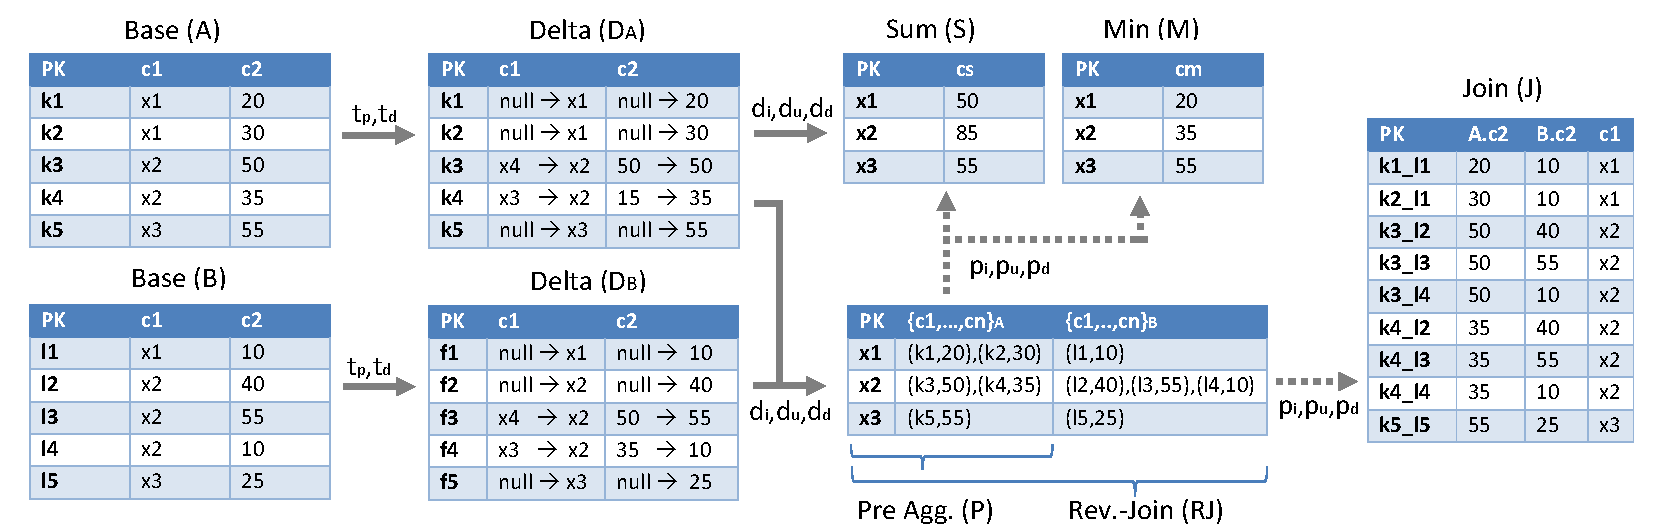
\includegraphics[width=\linewidth]{figures/ViewCalculationExample}
  \caption{View table example}\label{fig:view_table_example}
\endminipage\hfill
\end{figure*}
 
\noindent  
\textbf{Min and Max Views --} \texttt{MIN} and \texttt{MAX} views are
also aggregates. Both can be derived from a \texttt{DELTA} or a
\texttt{PRE-AGGREGATION} view. When derived from a \texttt{DELTA}
view, \texttt{MIN} and \texttt{MAX} are computed similar to a
\texttt{SUM}. However, a special case is the deletion of a minimum
(maximum) in a \texttt{MIN} (\texttt{MAX}). In that case, the new
minimum (maximum) has to be determined. Without the assistance of
auxiliary views, a table scan would have to be
performed~\cite{jacobsen:viewmaintenance}. This motivated us to derive
the \texttt{MIN} (\texttt{MAX}) from a \texttt{PRE-AGGREGATION}, which
prevents the need for a scan.  
%
%Let tables $A$, $D$ and $P$ be defined
%as before.  Then, a \texttt{MIN} view is defined as
%$M=\sigma_{Min(c_2)} (P)$. The \texttt{MIN} is updated as follows:
%%
%\begin{eqnarray}
%	p_{i/u} & \Rightarrow& put(S(v_1,\{\langle c_s, min(v_2, v_{2x_1},..,v_{2x_i})\rangle\}))\\
%	p_d & \Rightarrow& put(S(v_1,\{\langle c_s, min(v_{2x_1},..,v_{2x_i})\rangle\}))
%\end{eqnarray}



\subsection{Joins}
\label{subsec:common_views}


\noindent
\textbf{Join --} The \texttt{JOIN} view presents the results of $n$ 
joined base tables. Since the matching of join partners has been already 
completed in the \texttt{REVERSE JOIN} view, the \texttt{JOIN} view is 
used to display results in a proper way. To get the join result, the VM 
takes the output operations of the \texttt{REVERSE JOIN} view and 
multiplies their column families. Thereby, the \texttt{INNER}, 
\texttt{LEFT}, \texttt{RIGHT}, \texttt{FULL} join can be constructed. 

%Let the \texttt{JOIN} view be defined over the \texttt{REVERSE JOIN} 
%view as $J=\gamma^{-1}_{(K,L), map\langle K,c_2\rangle \times 
%map\langle L,c_2\rangle}(R)$. In Figure~\ref{fig:view_table_example} an example 
%of a \texttt{JOIN} view is depicted. We use notation $\gamma^{-1}$ to 
%indicate that the VM is doing the exact opposite of an aggregation at 
%this point. It takes two (or multiple) column families of a single row 
%and creates a set of result rows by building the cross product. While 
%building the cross product, the view manager combines the row keys of 
%both base tables to form a composite key ($(K,L)$). Likewise, it includes the 
%$c_2$ values of both base tables in the result. The update operations 
%are executed by the view manager as follows: 
%%
%\begin{eqnarray}
%		p_i,p_u& \Rightarrow& put(J(k_{x_1}l_{y_1},\{\langle c_1, v_{2x_1} \rangle,\langle c_2, v_{2y_j} \rangle\})),\\
%		 	&&...\notag\\
%		 	&&put(J(k_{x_i}l_{y_j},\{\langle c_1, v_{2x_i} \rangle,\langle c_2, v_{2y_j} \rangle\}))\\	
%		p_d& \Rightarrow& delete(J(k_{x_1}l_{y_1})),...,delete(J(k_{x_i}l_{y_1}))	 	 	
%\end{eqnarray}
%%
%\noindent 
%In order to build the different join types, the view manager varies
%the update computation as follows:
%{\renewcommand\labelitemi{}
%\begin{itemize}
%\setlength{\itemindent}{-.05in}
%\item \textbf{Inner}: Cross product $\{..\}A$ and
%  $\{..\}B$, neither $\{..\}A=\emptyset$ nor $\{..\}B=\emptyset$
%\item \textbf{Left}: Include rows with $\{..\}B=\emptyset$
%\item \textbf{Right}: Include rows with $\{..\}A=\emptyset$
%\item \textbf{Full}: Include rows with either
%  $\{..\}A=\emptyset$ or $\{..\}B=\emptyset$
%  \item \textbf{Equi}: Include rows with 
%  \item \textbf{Theta}: Include rows with
%\end{itemize}
%}


The good news is, with only a handful of manual
settings\footnote{Two of these, the {\texttt{\char'134 numberofauthors}}
and {\texttt{\char'134 alignauthor}} commands, you have
already used; another, {\texttt{\char'134 balancecolumns}}, will
be used in your very last run of \LaTeX\ to ensure
balanced column heights on the last page.}, the \LaTeX\ document
class file handles all of this for you.

The remainder of this document is concerned with showing, in
the context of an ``actual'' document, the \LaTeX\ commands
specifically available for denoting the structure of a
proceedings paper, rather than with giving rigorous descriptions
or explanations of such commands.

